\section{Robot Operating System 2 (ROS 2)}
\label{sec:robotoperatingsystem}

Robot Operating System (ROS) \citep{cit:quigley2009} merupakan kumpulan dari \emph{libraries}, \emph{drivers}, dan \emph{tools} yang mempermudah pengembangan sistem pada robot.
ROS memiliki \emph{command tool} seperti Linux, sistem komunikasi antar proses, dan berbagai macam \emph{packages} yang berhubungan dengan pengembangan sistem pada robot.
Proses yang dieksekusi pada ROS disebut sebagai \emph{Node}, komunikasi antar proses yang dimiliki menggunakan model \emph{publish/subscribe}, dan data komunikasi yang dikirimkan disebut sebagai \emph{Topic}.

\begin{figure} [ht]
  \centering
	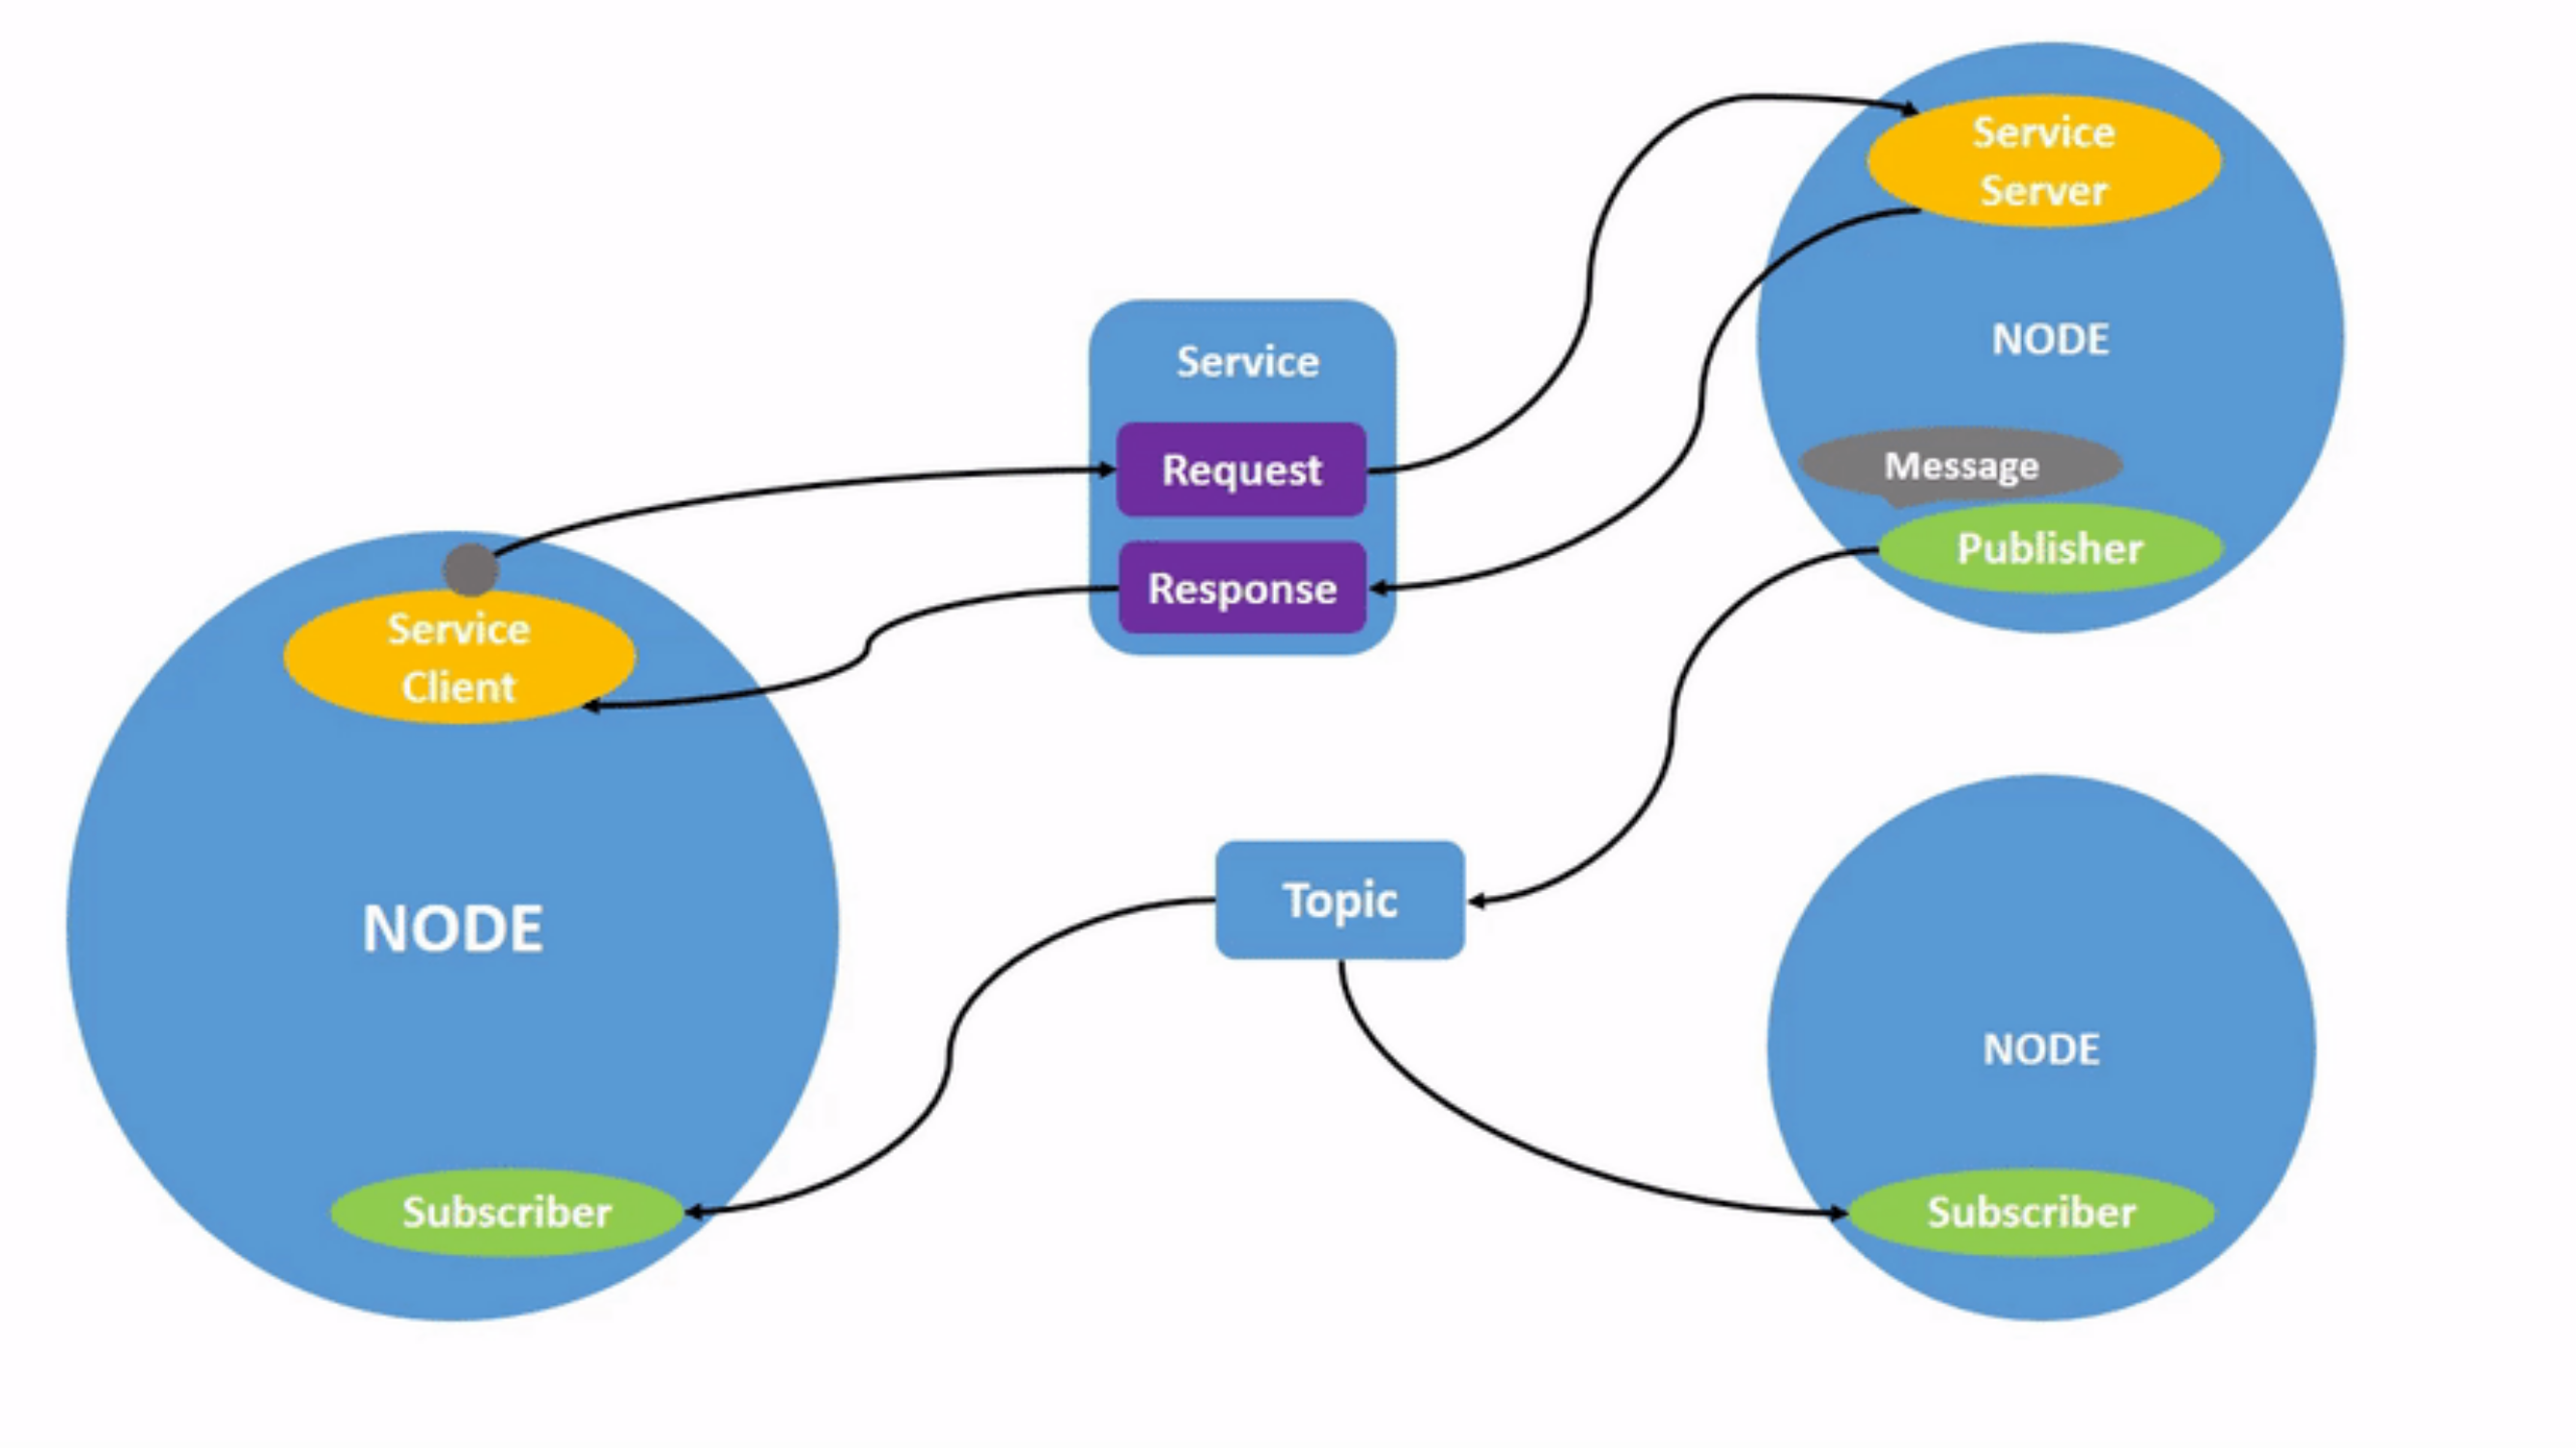
\includegraphics[scale=0.4]{gambar/komunikasi-ros.png}
	\caption{Diagram komunikasi antar node pada ROS 2 \citep{url:ros2nodes}.}
	\label{fig:komunikasiros}
\end{figure}

Seperti yang terlihat pada Gambar \ref{fig:komunikasiros}, Suatu proses \emph{Publisher} mampu mengirimkan satu maupun lebih \emph{Topic}, kemudian proses-proses lain yang melakukan \emph{subscribe} pada suatu \emph{Topic} bisa memperoleh isi dari \emph{Topic} tersebut.
Selain itu ada juga \emph{Sevice} yang memiliki fungsi seperti \emph{Topic}, hanya saja dilakukan secara dua arah.
\emph{Service} ini bekerja menggunakan model \emph{client/server} dimana \emph{Service Client} akan mengirimkan data permintaan dalam bentuk \emph{Request} dan kemudian \emph{Service Server} akan mengirimkan data balasan dalam bentuk \emph{Response}.

Generasi kedua dari Robot Operating System, ROS 2, merupakan kelanjutan dari ROS yang mengusung reliabilitas dan performa untuk penggunaan \emph{real-time} sembari masih mendukung keunggulan yang dimiliki oleh ROS sebelumnya \citep{cit:maruyama2016}.
Untuk memenuhi kebutuhan reliabilitas dan performa untuk penggunaan real-time tersebut, ROS 2 menggunakan Data Distribution Service (DDS) \citep{cit:castellote2003} \citep{cit:schlesselman2004}, standar industri untuk sistem komunikasi \emph{real-time} dan \emph{end-to-end middleware}, yang menggantikan sistem komunikasi antar proses yang dimiliki ROS sebelumnya.
